\documentclass[../main.tex]{subfiles}
\begin{document}
%qui ci metti gli autori che cita faure nell'articolo
The behavioural approach relates to the negotiators' behaviours. There are two main streams on which this approach is supported. The goal of the first one is to test the impact of culture on a series of behavioural variables in order to verify its actual influence. The second stream is based on surveys at describing the impact of culture on negotiators behaviours and subsequently at analysing its consequences.

Under the first stream, the first author mentioned is Carnevale: his article "Property, Culture, and Negotiation" approaches the issue under the individualist/collectivist cultural opposition. 
Then Kirkbride, Tang, and Westwood, with their article “Chinese Conflict Preferences and Negotiating Behaviour: Cultural and Psychological Influences”, provide us with an analysis of the Chinese approach to negotiation by highlighting the cultural context.
Then, Trompenaars gives his contribution to the topic by identifying seven cultural dimensions in his book "Riding the Waves of Culture: Understanding Cultural Diversity in Business". The last author quoted under the first stream is Hall: in his book "Beyond Cultures", in order to explain the influence of culture on negotiations he uses the dichotomy high-context and low-context cultural dimensions.

Under the second stream, the article mentioned is "The Influence of National Culture on Negotiating Style: A New Zealand-UK Perspective", written by Dr Anna Zueva, Dr Helen Rogers, Jemma Corbett, and Virginia Cathro. It analyses the influence of culture through a survey conducted on New Zealander and British negotiators. It appeals also to Hofstede's classification under his cultural dimensions: these are explained in Appendix 3. For further references, see "National Cultures in Four Dimensions: A Research-Based Theory of Cultural Differences among Nations" (1983).\\

The first author cited by Faure is Carnevale, particularly his article "Property, Culture, and Negotiation"(1995). In this article, Carnevale analyses property negotiations within their cultural context. Since, as we already said, culture is a broad concept, Carnevale focuses only on the individualist/collectivist paradigm\footnote{Individualist cultures focus on the individual's needs and aspirations, whereas collectivist cultures are group-oriented. Further explanations of these concepts will be given later on in the chapter.}. Indeed, his thesis put self-concept at the centre of the influence of culture on property negotiations. He argues that both individualism and collectivism can influence the preferences in the formula phase of a negotiation\footnote{For the concept of formula phase, see Chapter 2.}. Individualism also depends from the affluence of an individual; moreover, the number of groups available in a given society is important in determining the degree of individualism in a culture. Then, it is possible to say that individualism depends on: the number of available groups, the affluence of an individual, social mobility, and geographical mobility (if a person can change groups easily, then the group wont influence that individual much). Carnevale processes also the concept of allocentrism and idiocentrism, that, according to him, are intertwined with individualism and collectivism \autocite[312]{carnevale}. In particular, he asserts that allocentrism goes with a collectivist context because an allocentric person is more concerned about the well being of the community; whereas, in individualistic cultures, people are idiocentric, meaning they are self-driven.

Subsequently, Carnevale argues that there is a hypothetical relationship between the collectivism and individualism approach and the behaviour in negotiations. Particularly, Carnevale and other collaborators affirm that negotiators from a collectivist background are more attentive towards the nature of the relationship with the opposite party during the negotiation. As samples, they used individuals from Hong Hong (collectivist country) and the United States (individualistic country). The results showed that Hong Kong negotiators had more tendency to cooperate in negotiating with a friend than with a stranger \autocite[314]{carnevale}. This is because Asian cultures are relationship-oriented, thus once negotiators belonging to that culture have built a relationship with their counterpart, they will be more willing to negotiate. This is the reason why Hongkonger negotiators tend to cooperate more with a friend than with a stranger: because they already have a relationship with a friend, thus they trust their counterpart.

What emerges is that culture is seen as a mediator more than a moderator \autocite[321]{carnevale}\footnote{For the notion of mediator, see chapter 2.}. This is because cultural variables may have an impact on the outcome of the negotiation or an impact that is mediated by the strategies and tactics chosen by the parties (as shown in the picture below). That means that culture stands "in the way" between the negotiation and the negotiators' behaviours. It shapes and contributes actively to the negotiation, whereas a moderator has a neutral stance.

\begin{figure}[h]
    %\centering\includegraphics[width=0.8\textwidth]{images/cafoscari.png}
    \centering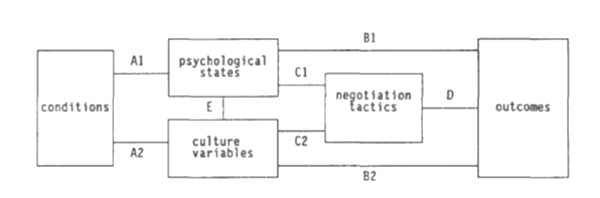
\includegraphics[width=0.65\textwidth]{images/carnevale.jpg}
    \caption{Carnevale's model.}
\end{figure}

Carnevale's point is that, according to him, it is not important to assess that people belonging to a culture adopt certain behaviours but, rather, what matters are the underlying theoretical processes that distinguishes the two parties on a relevant measure.\\

Another article cited by Faure in the first stream of the behavioural approach is “Chinese Conflict Preferences and Negotiating Behaviour: Cultural and Psychological Influences” (1991) written by Kirkbride, Tang, and Westwood. They analyse how Chinese cultural values influence the Chinese conflict resolution approach.

First of all, they define culture as the "means for, and the outcome of, attempts by people to locate and confer meaning upon their lives, experiences, events, and objects through the application of shared symbolic systems" \autocite[366]{tang}. They also determine the key aspects which can help understand Chinese value orientations. These consist of: harmony, collectivism, conformity, power distance, holism, contextualism, time, face, shame, reciprocity, and guanxi.

In Chinese culture, harmony between man and nature, man and man is derived from Confucianism. The focus is on keeping the relationships continuous and harmonious. 

Collectivism is connected to harmony because, in a harmonious world, the central point is the maintenance of the collectivity and issues are dealt in relation of their importance for the group.

Conformity is related to two Confucian principles. First, there are "rules of propriety" which frame relationships into five hierarchical dyads ('prince-minister', 'father-son', 'husband-wife', 'older brother-younger brother', 'senior friend-younger friend') and each individual is expected to behave according to these interpersonal relationships. Second, there is a principle according to which a human does not exist as a separate entity but is inevitably engaged within the context. Therefore, the individual will conform to the natural order of the relationships \autocite[367-368]{tang}. This will lead the individual in a conflicting situation to consider the relationship with others as the main factor. Indeed, usually, in a conflicting context, the person who is in a subordinate position in the relationship will be more likely to accommodate the person in a superior position.

Chinese culture is determined by an holistic view of life, and this can be mirrored in their approach in conflicting contexts. They have a high sensitivity to the context and tend to face the problem as a whole, instead of facing it little by little (as in Anglo-American cultures). This approach is connected with the harmonious view of life according to which issues are seen as a part of a whole.

Time is perceived as polychronic, repetitive, and associated with the events. They tend to deal with more issues at a time, contrarily to Western cultures\footnote{For further explanation of the concept, see Appendix 2 at the end of this chapter.}. 

Moreover, in Chinese culture, face is defined as an image of self determining attributes in terms of socially approved ones. Also, it is very shameful to interfere with group or interpersonal harmony. Indeed, shame is seen as an interpersonal frame in which a person's behaviour is compared to social norms rather than to assimilated personal standards. Thus, despite the tendency to avoid aggressive behaviour in conflictual context, there is the possibility of "shameful" behaviours.

Reciprocity is another universal principle that is significant in the Chinese culture. Indeed, they have the concept of favour (\textit{renging}) and reciprocation (\textit{pao}). In a negotiation, a concession made by one party is expected to be countered with a reciprocation of equal value by the other party.

Finally, the guanxi refers to the status of a relationship (including its intensity); therefore, in a collectivist society, a party will not only consider the relationship with the other party but will also consider the relationship with eventual third parties, in particular how they will perceive the behaviour of the negotiating parties.

In order to study how Chinese culture influences the negotiating processes of Chinese negotiators, the authors cite the Thomas model\footnote{For further references, see Thomas, Kenneth W. "Conflict and Conflict Management" in \textit{Handbook of Industrial and Organizational Psychology.} M. Dunnette (ed.), 889-935. Chicago: Rand McNally.} which identifies five different conflict-handling styles (competing, collaborating, compromising, avoiding, and accommodating).

\begin{figure}[h]
    %\centering\includegraphics[width=0.8\textwidth]{images/cafoscari.png}
    \centering
\includegraphics[width=0.40\textwidth]{images/thomas.png}
    \caption{Thomas model of conflict handling styles.}
\end{figure}

The authors suggest that conformity, harmony, collectivism, and shame create such pressure that lead Chinese negotiators not to show emotion and assertiveness in conflict situations. Thus, negotiators tend to compromise and to be avoidant. Moreover, the group-mindedness and relationship-centeredness induce negotiators to avoid confrontation and open competition. So do the holistic perspective and the fear of shame.\\

Another scholar who focused on culture and its dimensions is Trompenaars in his book "Riding the Waves of Culture: Understanding Cultural Diversity in Business."\footnote{He is also included under this approach because of his contribution to assess the reality of the cultural influence on negotiations.}. He borrows the definition of culture from Schein's book "Organisational Culture and Leadership"\footnote{See: Schein, E., \textit{Organisational Culture and Leadership}, Jossey-Bass, San Francisco, 1985.} in which culture is defined as the way in which a group of people solves problems and reconciles dilemmas. Trompenaars starts by providing a basis for cultural differences in explaining his point of view. According to him, cultural differences come from the different ways a culture approaches and solve a dilemma. Dilemmas can originate from three different situations: from the relationship with people; from the passing of time; and from environment-related context. By analysing the way in which cultures face problems withing these three categories, Trompenaars identifies seven cultural dimensions . The first category originates five of the mentioned dimensions \autocite[8]{trompenaars}.

\textbf{Relationship with people.} Trompenaars refers to five ways in which human beings relate to each other. To start, he takes inspiration from Parson's five relational orientations\footnote{See: Parsons, T., \textit{The Social System}, Free Press, New York, 1951.}.

\textit{Universalism vs Particularism.} In the universalist approach, there is the belief that there is a general principle that applies anywhere. In the particularist approach, far greater attention is given to the obligations of relationships and unique circumstances \autocite[9]{trompenaars}, the matter is about concrete reality rather than abstract codes. For example, in particularist cultures, a friendship is valued more: friendship may even come first than a better agreement. This can deeply shape the negotiators behaviours.

\textit{Individualism versus Communitarianism.} It corresponds to Hofstede's collectivism versus individualism or to Schwartz's embeddedness vs autonomy\footnote{For the explanation on Schwartz work, see Appendix 1 at the end of the chapter.}. In an individualist culture, there is a focus on the individual, therefore there is a tendency to concentrate on individuals' goals (even at the expenses of the community welfare). In communitarianism cultures, on the other hand, there is a tendency to strive for the community's interest. This opposition will reflect in a negotiator's behaviour when, for example, persuading the other party: in a collectivist culture, there might be the willingness to use rational reasoning because community interests are at stake.

\textit{Neutral versus Emotional.} In neutral cultures, the goal is to show very little emotion and be as similar to a machine as possible in order to be more efficient. Characteristic behaviours might be a controlled language where every word is weighted before being used and where social distance is wider. Examples of these cultures can be North American countries and North-Western European countries. The emotions are set aside as they are believed to confuse the issue. In emotional countries, expressing the whole spectrum of emotions is part of the negotiation process. This can be mirrored in using the whole body to communicate or to use less social distance in order to show better the emotions.

\textit{Specific versus Diffuse.} It relates to the approach of a negotiator towards their counterpart. Particularly, it relates to how much a negotiator puts themselves in the relationship with the other. In specific cultures, a negotiator will have the relationship prescribed by the contract. In diffuse cultures, the contact is more personal and a negotiator will put themselves as a whole in the relationship with their counterpart. Trompenaars provides us with an example: in a negotiation between North American and South American negotiators, the North Americans gave a well-thought presentation about their offer without respecting the South American diffuse approach. Then Swedish negotiators intervened, by getting to know the South American negotiators for over five days, then they offered a deal and, even though it was slightly less convenient than the one offered by the North Americans, the South American negotiators accepted. This indicates that a change in behaviour will also be a counterbalance for a disadvantaged situation in which negotiators have to top another deal made by other competing negotiators \mancite\autocite[9]{trompenaars}.

\textit{Achievement versus Ascription.} In the first case, the status of a person is gained with successful accomplishments. In the second one, the status is gained by birth, by blood, by kinship, by gender, by age, but also by connection or by educational record.

\textbf{Attitudes to time.} Time is also important in distinguishing different cultures. Particularly, the way a society looks at the concept of time. Indeed, in some cultures, there is a grater consideration for the past and the accomplishments achieved in there, such as the French culture: they give much value to \textit{ancien pauvre} opposed to the \textit{nouveau riche}. Contrarily, in some other cultures, there is focus on the accomplishments achieved in the present and what can be achieved in the future. One example is the American culture: Americans generally start from zero and what matters is their present performance and their plan to “make it” in the future \mancite\autocite[10]{trompenaars}. Moreover, in North American, Swedish, and Dutch cultures, time is perceived as a series of consecutive frames of events in a straight line. Whereas in other cultures, time is conceived in a circle in which the past and the present chase each other with some together with some future possibilities. The difference in the concept of time has a consequence on the choice of negotiation strategy. 

\textbf{Attitudes to the environment.} Cultural differences also come from the attitudes towards the environment and how it is conceived. In some cultures, values come from the individual and the surroundings are just a frame. In other cultures, the environment is conceived as something more powerful than individuals, almost as something to be feared or mirrored.

Each of these cultural dimensions have an impact on the negotiation process as negotiators from different cultural background will approach each of these above-mentioned dimensions. Some of them will have a bigger impact than others, but Trompenaars provides us with an all-around vision of how different aspects of the cultural dimensions actually influence the behaviours of the negotiators.\\

Edward Hall\footnote{Hall is included under this first stream because of his contribution in providing dimensions in which culture can influence the negotiators' behaviours.} was an anthropologist who provided some cultural dimensions in relation to cultural context, time, and space\footnote{In this analysis, only the cultural context will be examined: for further details on time and space, see Appendix 2 at the end of the chapter.}. 

In his book "Beyond Culture", he presents the differences between \textit{high context} and \textit{low context} cultures. He chose the law as a comparing basis to understand the contrast between the two different context for many reasons, but the main one is that "culture underlies the law, and many things can be read and understood by studying the way in which the law is handled" \autocite[107]{hall1}. From the way law is conceived and treated, he draws some characteristics that distinguish high context and low context cultures.

High-context cultures are characterised by use of non verbal communication, of implicit messages, of a solid distinction between the inner circle and the outer circle, of a inner locus of control. Time can be flexible and parties take time to negotiate as the process is more important than the outcome; there is a high commitment to long-term relationships. On the other hand, in low-context cultures, the locus of control is external, communication is based more on verbal language than body language, the distinction between inner circle and outer circle is not strong, in fact the group pattern changes if needed. There is low commitment to relationships and time is highly organised: in a negotiation, the outcome is more important than the process itself. Hall then compares these two types of context: by remaining in the legal framework, Hall highlights the difference between the French legal system (high context) and the North American one (considered low context within the legal framework). French contracts are much shorter than the American ones because, in the French system, information is available in the context and many concept are thought to be known by everyone. Contrarily, American contracts are long because in low context cultures nothing is taken for granted and in contracts there has to be an explanation of every principle that maybe in high context culture is thought superficial to be explained.

This difference can influence the behaviours of the negotiators. Indeed, negotiators from low-context culture take less time to negotiate, communication is straight and direct. Whereas high-context cultures' negotiators take time to negotiate and they use formal, refined language, their communication is not direct.

Hall shows us that this opposition fed by cultural differences has an effect on the outcome of the negotiation (in his example, within the law framework) to the extent that the actual material agreement has different lengths depending on which culture we are referring to.\\


Under the second stream, which is based on surveys at describing the impact of culture on negotiators behaviours and subsequently at analysing its consequences, the first article worth mentioning is "The Influence of National Culture on Negotiating Style: A New Zealand-UK Perspective", written by Dr Anna Zueva, Dr Helen Rogers, Jemma Corbett, and Virginia Cathro \footnote{This article is under this approach because it deals with the influence of culture through a survey.}. It provides an analysis of the negotiating style of negotiators from New Zealand and from the United Kingdom. They base their work mainly on Hofstede’s cultural framework\footnote{For Hofstede's work, see Appendix 3 at the end of the chapter}, but also on Hall's and Trompenaars’ works. They focus on nine characteristics of the negotiation style that might be influence by culture in the UK and New Zealand contexts. Those aforementioned characteristics are:
\begin{enumerate}
    \item The use of formal written or informal verbal contracts;
    \item Collaboration and competition in negotiations;
    \item Decision-making;
    \item The meaning and uses of time;
    \item Priorities in negotiation (deal- or relationship-focus);
    \item Importance of cultivating relationships;
    \item Attitudes towards negotiators’ status;
    \item Importance of structure in negotiations;
    \item Importance of long-term objectives;
    \item Willingness to disclose information during negotiations.
\end{enumerate}

The interviews were held with eight British and eight New Zealander sales managers. The respondents were searched mostly following a basis of equivalence and comparability. This means that the authors selected people to interview with a close match of background, education, occupation, demographic characteristics\footnote{The approach adopted by the authors was a qualitative semi-structured interview data collection approach. In fact, this kind of approach enables the researchers and the respondents to have a direct contact, thus reducing the possibility of a misunderstanding due to a potential miscommunication.
Because New Zealand and the United Kingdom are geographically distant, surveys were held by telephone. This method carries many advantages, such as: inexpensiveness, reasonably high response rates, high data quality (because respondents can clarify and provide evidence for their answers), and a relatively shorter time for collecting data. Nonetheless, this method has its disadvantages: indeed, a face-to-face connection is missing, hence important body language cues might be missed. Moreover, it was difficult to establish a close relationship by telephone.}.

Respondents were asked to formulate their answers on the basis of past negotiations in which they participated \autocite[10]{zueva}, that is their answers were based on personal experiences. Respondents were also free to suggest their own additional discussion topics.

The results showed both similarities and differences in the above-mentioned characteristics. The similarities were related to:

\textit{Use of formal written or informal verbal contracts.} Both nationalities ended the majority of their respective previous negotiations with verbal agreement even though a written document is needed for formal reasons. Indeed, while they feel comfortable ending an agreement with a verbal deal, they still necessitate the security of legal language and a written, signed contract.

\textit{Decision-making.} The respondents from New Zealand and from the United Kingdom had similar feedbacks related to decision-making practices in negotiations. In both cases, negotiators have consistent individual decision-making power. For example, negotiators were not required to ask for permission or approval of decisions to their superiors; indeed, there was not even the need to reach for consensus with other members of the organisation.

\textit{Attitudes towards negotiators’ status.} Moreover, the managers from both countries did not consider important the position of the negotiator as long as the person covering that position is able to make necessary decision on behalf of their company. These answers are consistent with the view of UK and NZ as individualist, low-power-distance, and achievement cultures \autocite[12]{zueva}.

\textit{Importance of Relationships.} Both people from New Zealand and from the United Kingdom revealed that they place much importance on building a relationship with the other party. However, the way the respondents described the relationships suggests that the nature of the relationships is at a superficial level. Moreover, the relationships were built for the purpose of the business negotiations and had nothing to do with personal attachments. In this way, what may have seemed an attitude related to collectivist, feminine values (according to Hofstede's scheme of values), it was indeed an endorsement of the view of the UK and NZ business culture as individualist, masculine, universalist, neutral, and specific \mancite\autocite[12]{zueva}.

\textit{Meaning of Time.} Time is conceived in a typically Western conception from both nationalities. Time carries a monetary value, therefore punctuality and schedules are necessary in order to be efficient. Time can also be seen as a negotiating tactic: some of the respondents replied "some clients are notorious for dragging out the negotiations and time wasting" and "you can use time in a negotiation for leverage" \mancite\autocite[13]{zueva}. Respondents also suggested the length of a negotiation. Managers from both countries agreed that a negotiation should not be rushed and that important negotiations require more time. Still, the main objective of the managers is to solve business issues rather quickly in order not to waste time. 

\textit{Reliance on Routines in Negotiation Process.} Managers from both the United Kingdom and New Zealand stated that they do not rely on specific routines during the negotiations and that they are comfortable in situations in which flexibility is required: that is, they feel able to adapt in unfamiliar situations if needed. Hofstede placed these two countries under the low uncertainty avoidance cultures and the results collected in this survey confirm this attitude carried by the two nationalities.

On the other hand, there were differences in the answers of the managers from the two countries. Those differences were related to:

\textit{Collaboration and Competition in Negotiation Approach.} In the answers of New Zealander managers it is possible to notice a trend: indeed, the answers provided show that managers from New Zealand favoured a collaborative approach to negotiations. Conversely, it is not possible to indicate a single, relevant trend in the British managers' responses. Indeed, most frequently they provided responses indicating both competitive approach and a combination of collaborative and competitive approach. The answers given by the British participants were in line with the description of British business culture as being individualist, masculine, and with an internal locus of control\footnote{The locus of control is the degree to which people believe that they have control over the outcome of events in their lives, as opposed to external forces beyond their control.}. The same does not hold, however, in the case of New Zealand, which is also considered as individualist, masculine, and internally-focused. New Zealander managers adopted a highly collaborative approach, which is more characteristic of collectivist, feminine cultures with an external locus of control \mancite\autocite[14]{zueva}. Possibly, the fact that New Zealand scores in a mid range in terms of masculinity in Hofstede's classification explains the collaborative behaviour. Nonetheless, the contradiction still stands because also the United Kingdom scores relatively low in Hofstede's classification. Although, this lack of consistency in the answers of British respondents might indicate that negotiators' behaviour is influenced by something else other than national culture (as it was mentioned in Chapter 3, Hofstede provides us with an explication of the different levels of cultures, such as generation, gender, ethnic, and more).

\textit{Short-Term versus Long-Term Goal Orientation.} By analysing the responses on the British managers, it was not possible to identify a specific trend if not that the managers agreed on focusing on long-term or short-term goals depending on the situation. Contrarily, the trend in the responses provided by the New Zealanders is clear: there is a preference on satisfying long-term goals over short-term goals. These results were not a surprise as Hofstede had already classified the United Kingdom as being more short-term oriented than New Zealand.

\textit{Priorities in Negotiations.} The United Kingdom and New Zealand have different priorities in negotiations. Indeed, on one hand, the British respondents' major concern was to close the deal and gain a profit from it; on the other hand, New Zealand was more focused on extracting a worthy relationship out of the negotiations. However, while in the British managers' responses, the trend was univocal and clear (to make a profit, to get a result), in the New Zealanders responses it was not possible to extract a single trend considering that the priorities varied and included achieving a win-win situation, making a good profit, completing negotiations within a certain time and budget, reaching a valuable agreement, retrieving information, building good relationships and focusing on the process rather than the outcome \mancite\autocite[15]{zueva}. While British responses are in line with Hofstede's classification (mentioned in the previous point), in the case of New Zealand it is not possible to assert the same due to the variation of responses.

\textit{Information Disclosure.} This is the point of greatest difference between the two nationalities. On one side of the spectrum, there is the United Kingdom: the British managers revealed that they disclose very little information. On the other side, New Zealanders were far more open to information disclosure, unless it was about a sensitive or confidential topic. Once more, the British responses match Hofstede's classification. However, New Zealander managers' responses provide no match with Hofstede's scores: indeed, New Zealand is considered, similarly to the United Kingdom, as an individualist, masculine, and with an internal locus of control. Therefore, questions arise as to whether differences in responses could be connected with differences between the UK and NZ individualism and masculinity scores \mancite\autocite[16]{zueva}.

The results of this study showed that there were some matches between the responses collected and Hofstede's classifications, but there also were some inconsistencies. Even though the United Kingdom and New Zealand are both classified as individualist and masculine in their decision-making practices and relationship orientation, New Zealander managers were significantly more collectivist and feminine in their use of collaboration in negotiations. This can be explained by the fact that even if in Hofstede's classification the two countries have a little difference in scores, this little difference equals a large difference in cultures. Moreover, it could be either that the dimensions of individualism, masculinity and locus of control predict better some behaviours, such as the concern about relationship, than others, such as competitive of collaborative approaches; or that those dimensions are not good predictors of behaviour in negotiations and other factors should be considered \mancite\autocite[19]{tang}.\\

It is possible to see how culture has an impact on negotiations, even under point of view that one might consider far from the negotiation context. Each of the authors mentioned provided us with tools in order to understand in which way the cultural background can influence the timing, the pace, the language of a negotiation process.
\pagebreak

\subsection*{Appendix 1: "A Theory of Cultural Value Orientations", Schwartz.}

One author that is worth mentioning within the cultural dimension context is Schwartz and his article "A Theory of Cultural Value Orientations" in which he describes three dimensions within which he places seven values. He identifies values that counterbalance each other: \textit{embeddedness} versus \textit{autonomy} (which correspond to Hofstede's collectivism versus individualism), \textit{hierarchy} versus \textit{egalitarianism}, and \textit{mastery} versus \textit{harmony}. Moreover, he distinguishes between intellectual and affective autonomy (hence, the seven values): the former relates to the attitude of individuals to pursue their own; the latter encourages individuals to seek positive experiences for themselves. The following figure shows the values related to these dimensions:

\begin{figure}[h]
    %\centering\includegraphics[width=0.8\textwidth]{images/cafoscari.png}
    \centering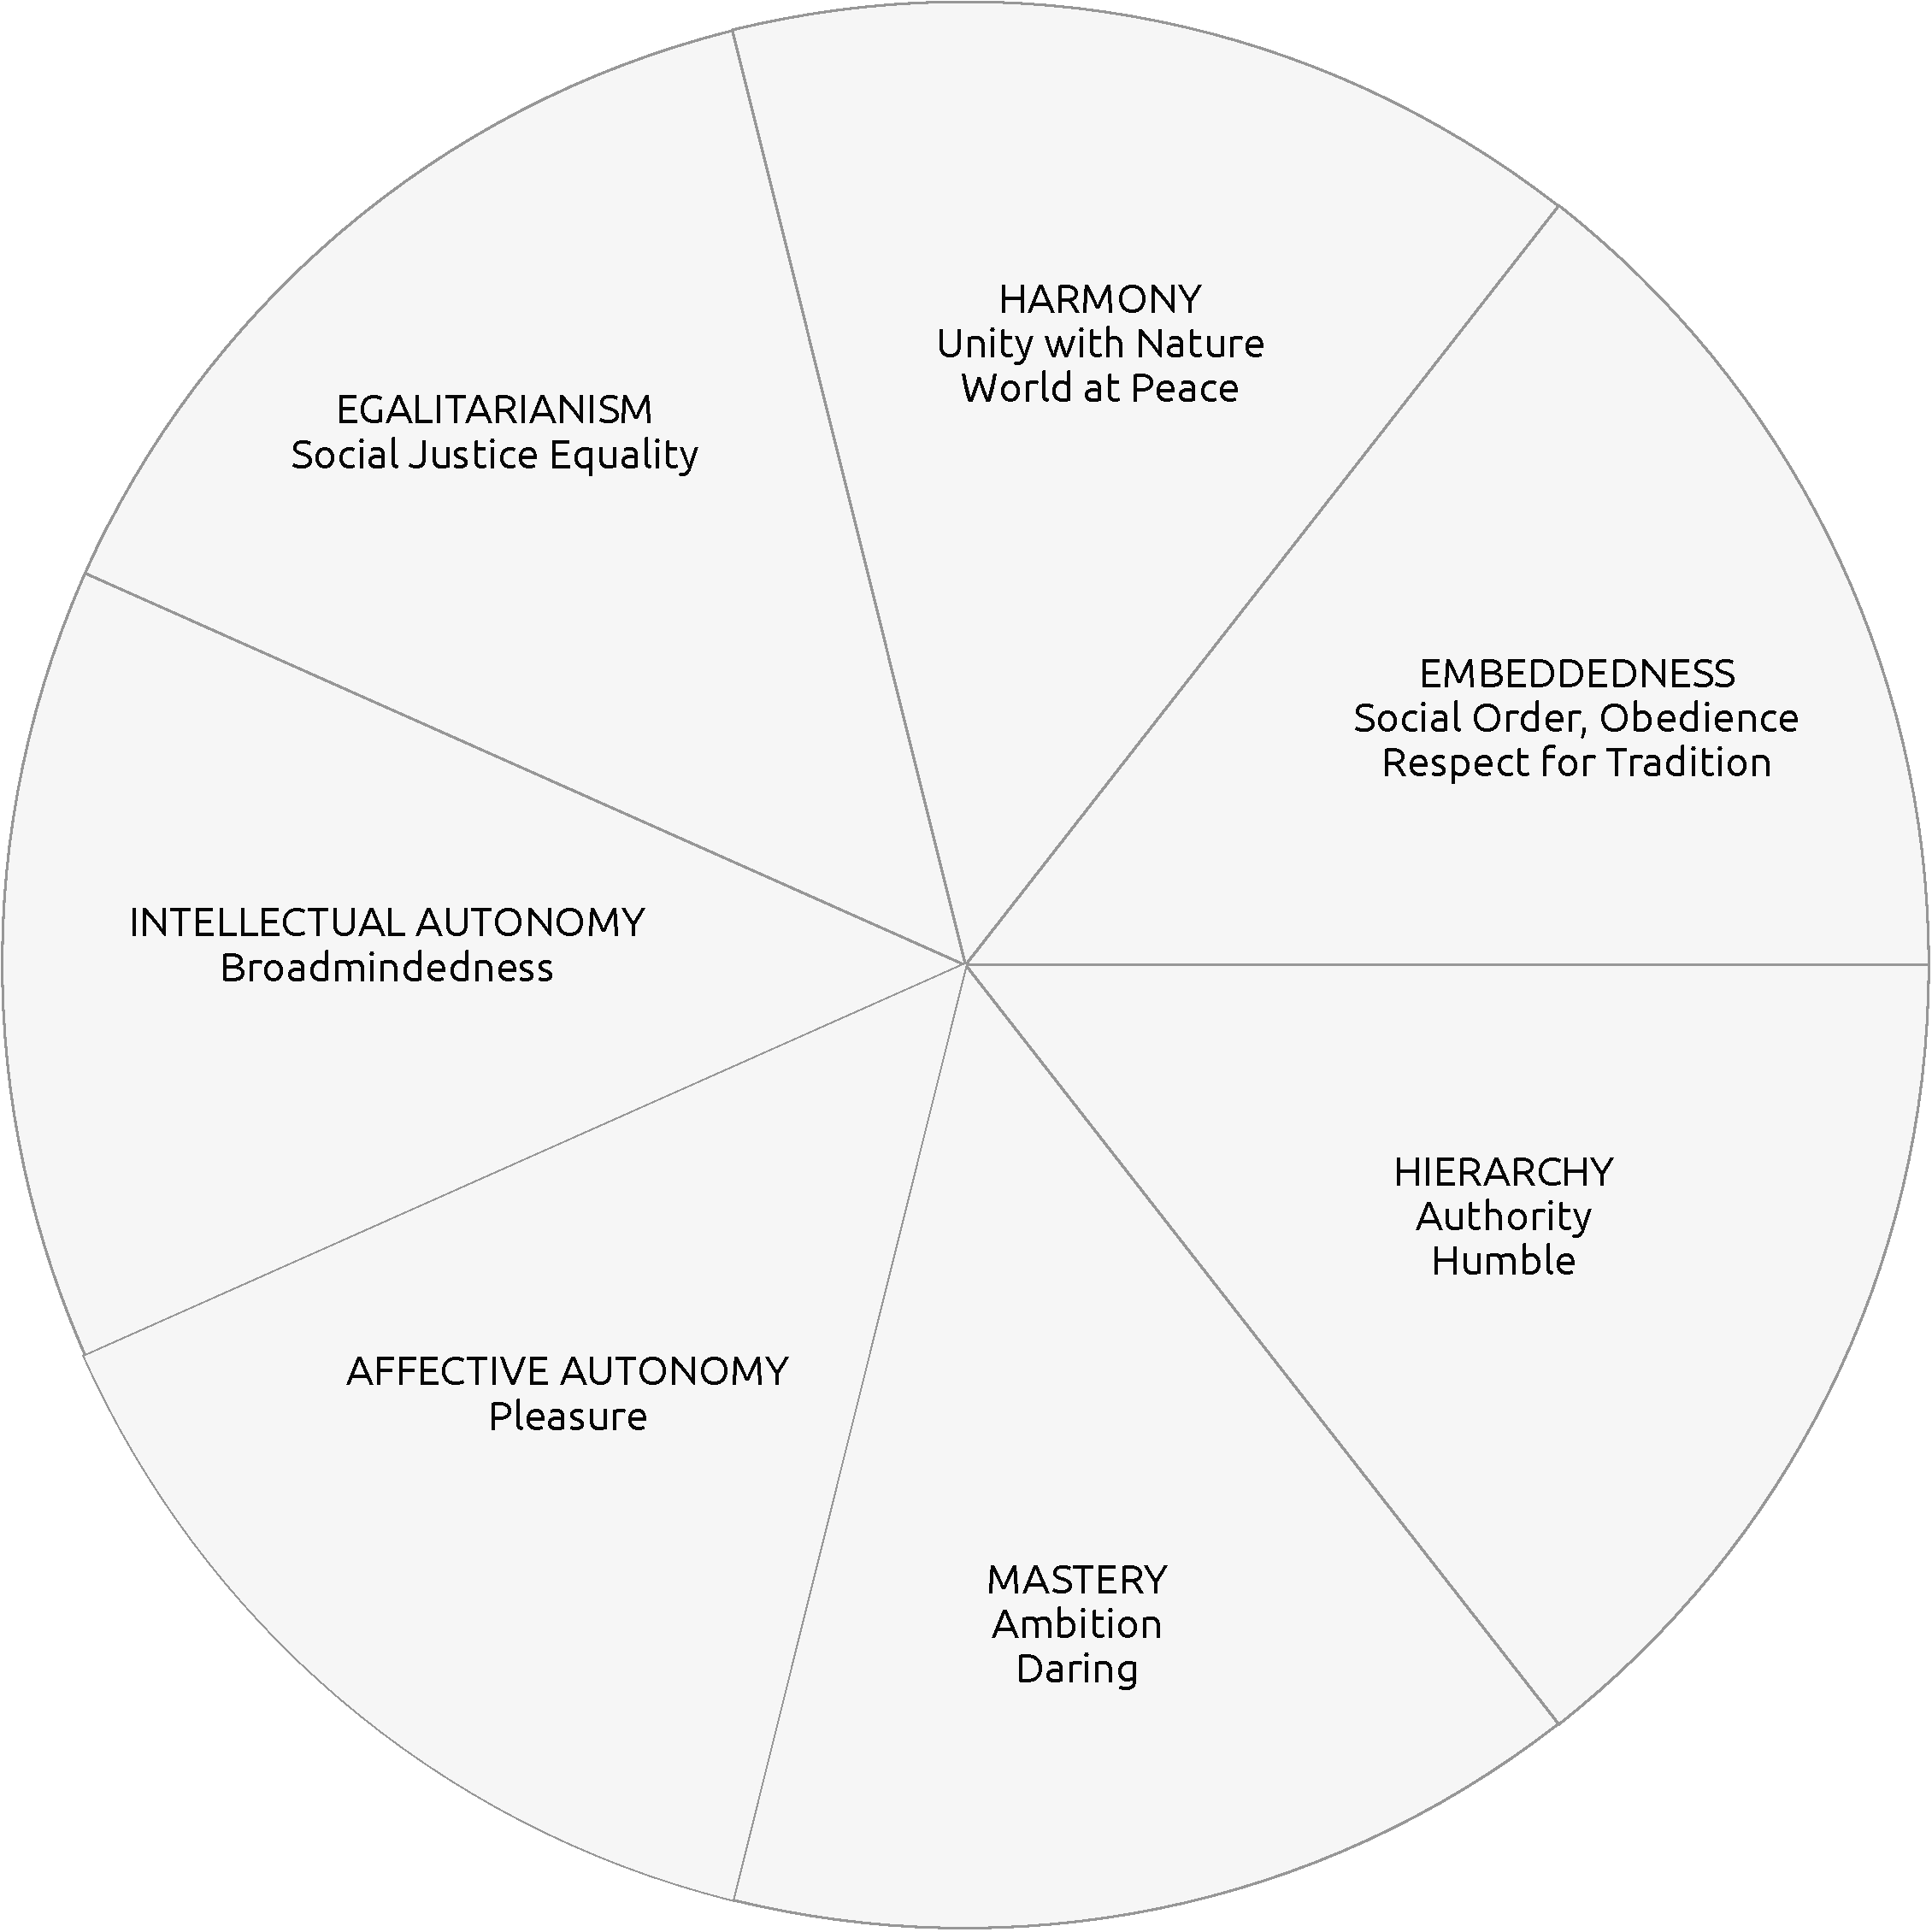
\includegraphics[width=0.3\textwidth]{images/socialvalues.pdf}
    \caption{Schwartz's seven values.}
\end{figure}

In autonomy, people are seen as autonomous and they are encouraged to express their ideas, values, emotions and to embrace their unique selves. In embeddeness, people are seen in function of the collectivity and the life of the individuals finds meaning in the collectivity, in the relationship with others, in the pursuit of the same goals. In a society as such, it is important to maintain the status quo otherwise the traditional order might be altered and the in-group harmony might be spoiled. In an egalitarianism driven society, people are encouraged to acknowledge the other individuals as a moral equals and to care for everyone's welfare. On the other hand, hierarchy ensures a productive, responsible behaviour. There is an unequal distribution of power; people will attain to the rules going with their roles. Harmony refers to the tendency to live in the world as it is, without changing it. Whereas mastery relates to the fact that individuals tend to shape the natural and social environment according to their agenda.


\subsection*{Appendix 2: "Dance of life", Hall.}

In his book "Dance of life", Hall provides us with an explanation of the concept of time across cultures. Indeed, Hall distinguishes between monochronic time and polychronic time, explaining that a considerable amount of bitterness between people of different cultures occurs due to different conceptions of time \autocite[179]{hall2}. In monochronic cultures, time is conceived as something linear in which action are put in a sequence. Therefore, events are planned to happen one at a time. In this context, efficiency is measured through the use of time. People in monochronic culture are committed to the job, need information as they are usually in a low context culture, are not prone to change plans, and are used to short-term relationships. Conversely, In polychronic cultures, time is conceived as a simultaneous manifestation of many events. People in this context are embedded in high context cultures, easily change their plans, commit to building long-term relationships with people, and tend to borrow and lend things much more.\\

Hall is arguably the pioneer of proxemics, which is a part of the study of non verbal language that analyses the "symbolic and communicative role in a culture of spatial arrangements and variations in distance, as in how far apart individuals engaged in conversation stand depending on the degree of intimacy between them"\footnote{According to the definition of Dictionary.com}. In the book "The Hidden Dimension", we are provided with the differentiation of a person's space of interaction. Particularly, Hall distinguishes between intimate, personal, social, and public distance.

In the intimate distance, the presence of another person is unmistakable as it reaches a maximum of 45 centimetres away from the person. It is divided between \textit{close phase} and \textit{far phase}. The former refers to a distance of love-making or wrestling. At this distance, the use of distance receptors is highly reduced aside of the sense of smell and touch. Also vocal communication is reduced and  the vocalisations that occurs are mainly involuntary. The latter refers to the situation in which two people are brought together but thighs and pelvis are not touching (contrarily to what happens in the close phase), though hands can reach the other person's body. The peripheral vision includes the outline of the head and the shoulders.

The personal distance can take up to 1.2 meters and it relates to social events or with interactions with friends. Also this space is divided in \textit{close phase} and \textit{far phase}. In the close phase, bodies are a little further from each other than in the intimate distance, however the personal space is occupied by people close to the the person as it is easy to grasp one's arm and to see clearly the facial feature and the muscles surrounding the eyes. The far phase is the situation in which two people cannot easily touch each other anymore. It is the "limit of physical domination"\autocite[120]{hall3} as beyond this area it is not possible to touch each other anymore. Still, details in the other person's face are detectable and sometimes even breath odour can be perceived.

The social distance can be up to 3.6 meters wide and relates to social situations such as meetings. As the two precedents areas, this too is divided in \textit{close} and \textit{far phase}. In the close phase, impersonal business occurs and usually people who work together stand in this area. This distance is also very common for people attending casual social events. The far phase has a more formal character: the desk of an important person is wide enough to reach the far phase of the social distance with the interlocutor. The eyes and the mouth are in the focal point of vision. Also, the voice level is remarkably higher than the close phase.

In the \textit{close phase} of public distance, the voice is loud but it is not at a full volume. Face details are no longer visible: the eyes cannot be seen and also the body loses its multidimensionality by looking flat instead. The \textit{far phase} is set around public important figures. However, it is also used in public occasions by people and also by actors during performances. Voice and expressions have to be exaggerated to be noticed by the public.  

\begin{figure}[h]
    %\centering\includegraphics[width=0.8\textwidth]{images/cafoscari.png}
    \centering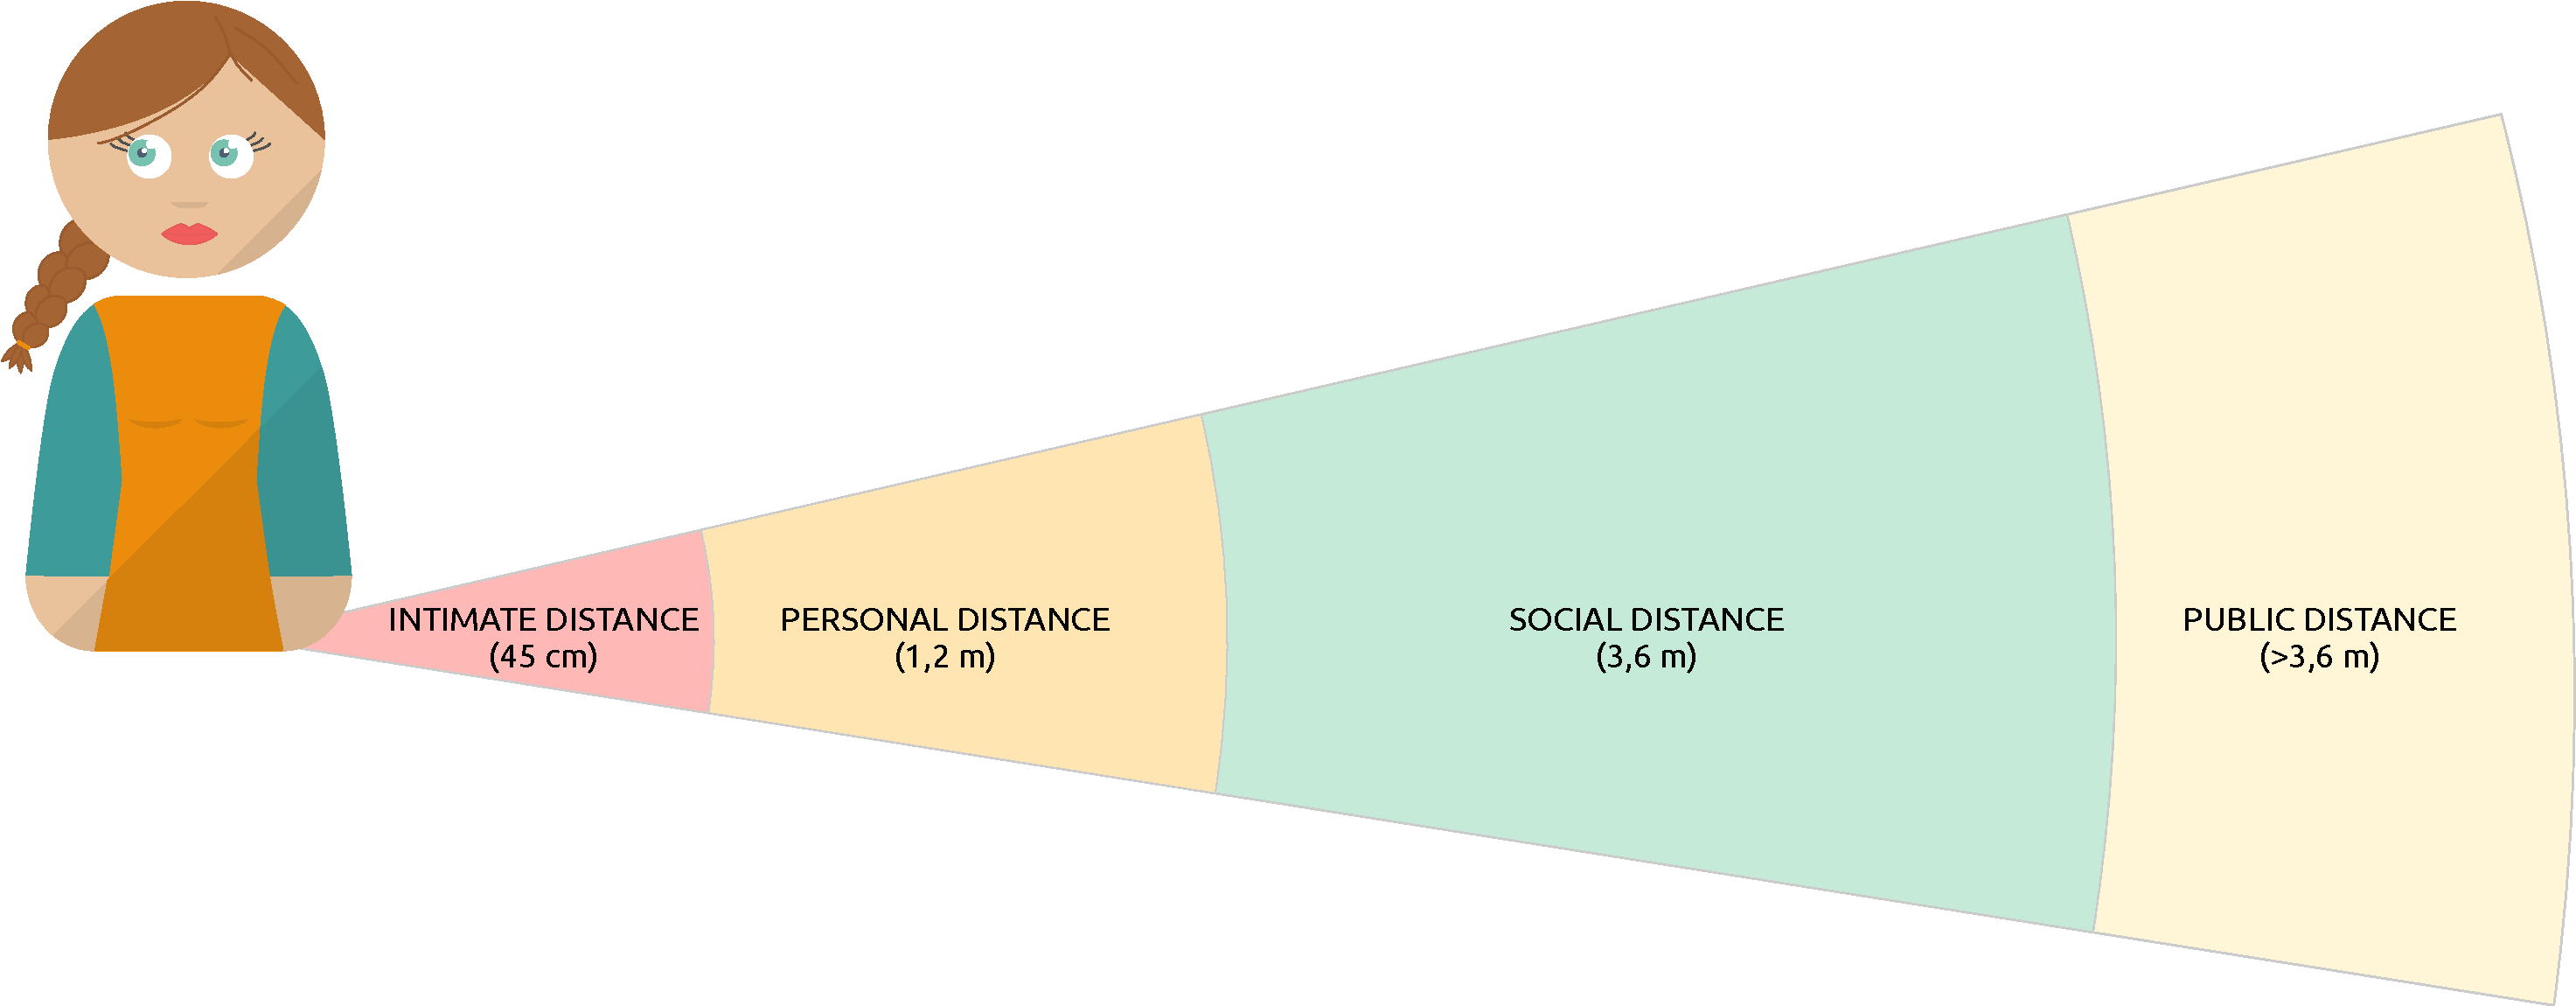
\includegraphics[width=0.65\textwidth]{images/anna.pdf}
\end{figure}
\pagebreak

\subsection*{Appendix 3: "National Culture in Four Dimensions, A Research-based Theory of Cultural Differences among Nation", Hofstede.}

Hofstede, for this article, collected questionnaire data from 67 countries and tried to extrapolate an analysis. The result was the identification of four dimensions that might help to develop hypothesis in cross-cultural studies. These dimensions can be applied to social systems and not on the individuals belonging to them.
\begin{enumerate}
\item \textit{Power distance}: relates to authority ranking; particularly, society's way of dealing with power relationships is established through the values of superiors as well as of subordinate; %cerca fonteeeeee
\item \textit{Uncertainty avoidance}: concerns the tendency to avoid situations that do not have a clear and certain outcome or that cause stress.
\item \textit{Individualism versus collectivism}: involves the degree by which a culture promotes goals from which individuals can benefit, rather than goals for which the individual is dependent from a collectivity. %riguarda che fa un po' cacare
\item \textit{Masculinity versus femininity}: relates to the tendency of people to be inclined towards values considered more masculine or feminine. Masculine cultures promote assertiveness, individualism, competitiveness. Feminine cultures foster cooperation, collectivism.
\end{enumerate}

\end{document}